\documentclass[../sotsu.tex]{subfiles}

\graphicspath{{../fig/}}

\begin{document}


\section{集合・写像}

\subsection{集合}
\label{sec:set-intro}

すべての数学の基礎となるのが「集合」である.
この節では集合を扱ううえで必須である用語を素朴に導入する.

「集合」をきちんと定義するのは難しいが,ここでは以下のように考える.

ある特定の性質をもつモノの集まりを\word{集合}(set)という.
集合とは単なるモノの集まりではなく,何が集まっているかを定められる集まりである\cite{uchida-set-2020}.

\begin{example}
    「\textgt{正の実数の全体}」「\textgt{ひらがなの全体}」「\textgt{名大付属図書館の蔵書全体}」には,それぞれ何が入っていて,何が入っていないのかを定められるので集合である%
    \footnote{
        もちろん「ひらがなの全体」に変体仮名を含むのか,「名大付属図書館の蔵書全体」はいつの時点の蔵書を指すのかは決めておく必要がある.
    }.
    一方で,「\textgt{絶対値の小さな複素数の全体}」「\textgt{難しい漢字の全体}」「\textgt{偉大な物理学者の全体}」には,何が入っていて何が入らないのかを客観的に定められないので,集合とは言わない%
    \footnote{
        ``偉大な物理学者''を「ノーベル物理学賞の受賞者」と定義すれば,「\textgt{偉大な物理学者の全体}」は集合になる.
        しかし,そうであればはじめから「\textgt{ノーベル物理学賞の受賞者の全体}」といえばよいし,
        そもそも偉大な物理学者≠ノーベル物理学賞受賞者であるのは物理学を学んだ人ならよく理解していることだろう.
    }.
\end{example}

$X$をある集合とする.$X$を構成するモノのことを,$X$の\word{元}[げん](element)あるいは\word{要素}[よう|そ]という.
$a$が$X$の元であるとき,「$a$は$X$に属する」あるいは「$a$は$X$に含まれる」といい,$a \in X$とかく.
$a$が$X$の元でなければ,$a \notin X$とかく.
$X$と$a$の位置を入れ替えて$X \ni a$あるいは$X \nni a$とかいてもよい\cite{uchida-set-2020}.

\begin{example}
    $X$を「\textgt{愛知県にある市の全体}」とすると,$X$は集合である.
    このとき,\textgt{名古屋市}は$X$に属する(含まれる)ので,$\text{\textgt{名古屋市}} \in X$とかく.
    一方,\textgt{\ruby{四日市}{よっ|か|いち}市}は$X$に属さない(含まれない)ので,$\text{\textgt{四日市市}} \notin X$とかく.
    ほかにも
    \begin{equation*}
        \textgt{豊田市} \in X,
        \qquad
        \textgt{浜松市} \notin X,
        \qquad
        \textgt{\ruby{飛島}{とび|しま}村} \notin X
    \end{equation*}
    といったふうに,それぞれ$X$に含まれるか含まれないかを決定できる.
\end{example}

任意の集合$A$と任意の$x$に対して,$x \in A$と$x \notin A$のいずれか一方が必ず成り立つ.

集合を表すのには,いくつかの方法がある.
まずは$\{ 1, 2, 4 \}$のように\ruby{波括弧}{なみ|かっ|こ}(brace)の中に元を書き並べる方法である.
しかし,この書き方だと無限個の元を含む集合,たとえば「\textgt{自然数全体の集合}$\symbb{N}$」を表すことができない.
そこで,
\begin{equation*}
    \symbb{N} = \Set{  x  \given  \text{$x$は自然数}  }
\end{equation*}
のように縦棒$|$を書き,その前に含むべき元,うしろに元が含まれる条件をかく.
たとえば$\Set{  x \in \symbb{N}  \given  x > 2^{10}  }$とかけば,これは$2^{10}$より大きい自然数の集合を表す.

集合の表記になれるため,また今後のための準備もかねて,数の集合をいくつか挙げておこう.
\begin{subequations}
    \label{eq:number-sets}
    \begin{align}
        \text{自然数全体の集合} \, \symbb{N} &= \Set{  1, 2, 3, \dotsc  }
        \\
        \text{整数全体の集合}  \, \symbb{Z} &= \Set{  \dots, -2, -1, 0, 1, 2, 3, \dotsc  }
        \\
        \text{有理数全体の集合} \, \symbb{Q} &= \Set*{  \frac{p}{q}  \given  p \in \symbb{Z}, \  q \in \symbb{N}  }
        \\
        \text{実数全体の集合}  \, ℝ &\phantom{=}
        \\
        \text{複素数全体の集合} \, ℂ &= \Set{  a + b \iu  \given  a, b \in ℝ  }
    \end{align}
\end{subequations}

これに倣って,
\textgt{正の実数全体の集合}は,$\Set{  x \in ℝ  \given  x > 0  }$とかける.

元をひとつも含まない集合$\{ \; \}$を考えることもできる.
このような集合を\ruby[<->]{空集合}{くう|しゅう|ごう}とよび,
特別に記号$\emptyset$を使ってあらわす\footnote{ギリシャ文字の$\phi$を使う人もいる.}.


\subsubsection*{集合の関係}

いままで1つの集合について扱ってきたが,
ここで2つの集合の関係についてみてみよう.
集合$X$と集合$Y$について,$X$のすべての元と$Y$のすべての元が一致するとき,
$X$と$Y$は\word{一致する}といい,
$X = Y$とかく.
集合$X$と集合$Y$について,$Y$のすべての元が$X$の元であるとき,
$Y$は$X$に\word{含まれる}(あるいは$X$は$Y$を含む)といい,
$Y \subset X$とかく.

「含まれる」ということばと反するが,
定義から$X = Y$のときも$X \subset Y$が成り立つ.
集合$X$と$Y$が一致することを直接示すかわりに
$X \subset Y$かつ$X \supset Y$を示すことで,$X = Y$といえる.

たとえば,$X = $

$X$の元であるか$Y$の元であるものすべてを集めた集合を,
\word{和集合}[わ|しゅう|ごう]あるいは\word{合併}[がっ|ぺい]といい,
$X \cup Y$とかく.
$X$の元であり,かつ$Y$の元でもあるものすべてを集めた集合を,
\word{共通部分}[きょう|つう|ぶ|ぶん]あるいは\word{交わり}といい,
$X \cap Y$とかく.

特に$X$と$Y$の元がかぶっていないとき,
和集合$X \cup Y$のことを$X \sqcup Y$とかいて,
\word{非交和}[ひ|こう|わ]あるいは\word{直和}[ちょく|わ]ということがある.



\subsection{集合の演算}

\cref{sec:set-intro}で素朴に導入した集合を,
もう少し形式的なところに注目して調べてみよう.


% 空集合
% %%%%%%%%%%%%%%%%%%%%%%%%%%%%%%

\begin{definition}
    \label{dfn:empty-set}
    元をひとつも持たない集合$\{ \; \}$を\word{空集合}[くう|しゅう|ごう]\index{くうしゆうこう@空集合}といい,
    記号$\emptyset$であらわす.
\end{definition}

数学において存在が保証されている唯一のものが空集合である.


% 集合族
% %%%%%%%%%%%%%%%%%%%%%%%%%%%%%%

\begin{definition}
    \label{dfn:family-of-sets}
    集合からなる集合を\word{集合族}[しゅう|ごう|ぞく][しゆうこうそく](family of sets)という.
\end{definition}

たとえば,
$\ab\big\{ \{ \ \}, \  \{ 1 \}, \  \{ 1, 2 \}, \  \{ 1, 2, 3 \}  \}$は集合族である.

元が集合である集合に対して名前がついているのは,
単にそのような集合をよく扱うからである.


\begin{definition}
    \label{dfn:indicator-function}
    集合$A$に対し,
    \refdfn[写像]{dfn:map}$\chi_A \colon A \to \{ 0, 1 \}$を
    \begin{equation}
        \chi_A (x) \coloneq 
        \begin{cases}
            1  &  \text{if } x \in A  \\
            0  &  \text{if } x \notin A  \\
        \end{cases}
    \end{equation}
    で定める.
    $\chi_A$を,集合$A$の\word{定義関数},
    \word{特性関数}(characteristic function),
    あるいは\word{指示関数}(indicator function)という.
\end{definition}




% 包含
% %%%%%%%%%%%%%%%%%%%%%%%%%%%%%%

\subsubsection*{集合の包含}

集合$Y$が集合$X$を含むということは,
次のように定式化される.

\begin{definition}
    2つの集合$X, Y$の\ruby{包含}{ほう|がん}関係を,
    次のように定義する.
    \begin{enumerate}
        \item 任意の$x \in Y$に対し,$x \in X$が成り立つとき,
            \word{$X$は$Y$を含む}\index{ふくむ@含む},
            あるいは\word{$Y$は$X$に含まれる}といい,
            $X \supset Y$または$Y \subset X$とかく.
        \item $X \subset Y$かつ$Y \subset X$のとき,
            \word{$X$と$Y$は一致する}といい,
            $X = Y$とかく.
        \item $X \subset Y$かつ$X \neq Y$のとき,
            特に$X \subsetneq Y$とかく.
    \end{enumerate}
    $Y$が$X$を含まないとき,$Y \not\subset X$または$Y \not\supset X$とかく.
\end{definition}

以下は明らかである.

\begin{proposition}
    集合$X, Y, Z$について,
    $X \subset Y$かつ$Y \subset Z$なら,
    $X \subset Z$が成り立つ.
\end{proposition}




\subsubsection*{集合の演算}

\begin{definition}
    \label{dfn:union-of-set}
    \label{dfn:intersection-of-set}
    $X, Y$を集合とする.
    2つの集合の$X \cup Y$を,
    \begin{equation}
        X \cup Y  \coloneq  \Set{  x  \given  x \in X \, \text{または} \, x \in Y  }
    \end{equation}
    \word{和集合}[わ|しゅう|ごう](union)\index{わしゆうこう@和集合},
    あるいは\word{合併}[がっ|ぺい]\index{かつへい@合併}という.
    2つの集合の$X \cap Y$を
    \begin{equation}
        X \cap Y  \coloneq  \Set{  x  \given  x \in X \, \text{かつ} \, x \in Y  }
    \end{equation}
    を\word{共通部分}[きょう|つう|ぶ|ぶん](intersection)\index{きようつうふふん@共通部分},
    \word{交差}\footnote{
        \ruby{交叉}{こう|さ}とも書く.
        \cref{footnote:joyo-kanji}(\cpageref{footnote:joyo-kanji})を参照.
    },あるいは\word{交わり}という.
\end{definition}

\begin{definition}[非交和]
    \label{dfn:disjoint-union}
    $X \cap Y = \emptyset$であるとき,
    和集合$X \cup Y$を特に\word{非交和}[ひ|こう|わ][ひこうわ](disjoint union)
    あるいは\word{直和}[ちょく|わ][ちよくわ](direct sum)といい,
    $X \sqcup Y$,$X \amalg Y$などとかく.
\end{definition}



% 冪集合
% %%%%%%%%%%%%%%%

集合論ではある``普遍集合''の部分集合がよく登場する.
部分集合を扱う上で便利であるのが冪集合である.

\begin{definition}
    \label{dfn:power-set}
    $X$を集合とする.
    $X$の部分集合すべてを元として含む集合を,
    $X$の\word{冪集合}[べき|しゅう|ごう][へきしゆうこう](power set)といい%
    \footnote{略字で``\ruby{巾}{べき}集合''とかくことも多い.},
    $\symcal{P}(X)$,$\symfrak{P}(X)$,$2^X$などとかく%
    \footnote{
        $\symcal{P}$,$\symfrak{P}$はいずれもアルファベットのPである.
    }.
\end{definition}

たとえば,
$X = \{ a, b \}$とすると,
$\pset(X) = \ab \big \{ \emptyset, \  \{ a \}, \  \{ b \}, \  \{ a, b \}  \}$である.

部分集合$A \subset X$と\refdfn-[指示関数]{dfn:indicator-function}$\chi_A$が1対1に対応するので,
$N$個の元をもつ集合$X$の冪集合は,$2^N$個の元をもつ.
これが$2^X$という表記の理由である.




% %%%%%%%%%%%%%%%%%%%%%%%%%%%%%%%%%%%%%%%%%%%%%
% 写像
% %%%%%%%%%%%%%%%%%%%%%%%%%%%%%%%%%%%%%%%%%%%%%

\subsection{写像}
\label{sec:map}

ある集合の\ruby{元}{げん}(要素)と別の集合の元を結びつける規則のことを写像という.
数学の基礎を作る重要な概念である.
特に\ruby{圏論}{けん|ろん}とよばれる数学の一分野では,
集合ではなく写像(射)のほうが主役である.

物理学において写像をあらわに意識することはあまりないが,
例えば量子状態を記述する`関数'は写像の一種であるし,
また,微分・積分というのは関数と関数を結びつける写像である.
さらには\cref{sec:operator}で扱う\ruby{演算子}{えん|ざん|し}も,
写像の一般化としてみることができる.

\begin{definition}[写像]
    \label{dfn:map}
    $X, Y$を集合とする.
    $x \in X$に対して,ある$y \in Y$を対応付ける規則のことを,$X$から$Y$への\word{写像}[しゃ|ぞう](map)という.
    
    $f$が$X$から$Y$への写像であることを,$f \colon X \to Y$とあらわす.

    $X$を$f$の\word{定義域}[てい|ぎ|いき](domain),$Y$を$f$の\word{終域}[しゅう|いき](codomain)という.
\end{definition}

\begin{example}
    $X = \{ 1, 2, 3 \}$,$Y = \{ a, b, c \}$とする.
    次のように定義された$f$は$X$から$Y$への写像である.
    \begin{subequations}
    \label{eq:3-to-3-map-example}
    \begin{alignat}{3}
               f(1) &= a, 
        &\quad f(2) &= b, 
        &\quad f(3) &= c.
    \end{alignat}
    また,次のような$g$および$h$も$X$から$Y$への写像である.
    \begin{alignat}{3}
              g(1) &= c,
        &\quad g(2) &= c,
        &\quad g(3) &= a.
        \\
              h(1) &= a,
        &     h(2) &= a,
        &     h(3) &= a.
    \end{alignat}
    \end{subequations}
\end{example}

\begin{example}
    $X = \symbb{N}$,$Y = \symbb{N}$とする.
    $x \in X$に対して,$y \in Y$を
    \[ y = f(x) = 3x \]
    で定めたとき,$f$は$\symbb{N}$から$\symbb{N}$への写像である.
    簡単のために
    \[ X \ni x \longmapsto 3x \in Y \]
    とかくこともある.
\end{example}

\begin{example}
    $X = ℝ$,$Y = ℝ$とする.
    $x \in X$に対して,$y \in Y$を
    \[ y = f(x) = x^2 \]
    で定めたとき,$f$は$ℝ$から$ℝ$への写像である.

    $ℝ$から$ℝ$への写像や$ℂ$から$ℂ$への写像を,特に\word{関数}[かん|すう](function)という.
\end{example}

\begin{definition}[像]
    \label{dfn:image}
    $f \colon X \to Y$を写像とする.
    集合
    \begin{equation}
        \image f  \coloneq  \Set{ f(x) \in Y  \given  x \in X }
    \end{equation}
    を$f$の\word{像}[ぞう](image)という.
\end{definition}

$f$の像を\word{値域}[ち|いき](range)ということもある.
$f$の値域といった場合,$f$の終域を指すことも像を指すこともあり,注意が必要である.

\begin{definition}[部分集合の像]
    $f \colon X \to Y$を写像とする.
    部分集合$A \subset X$に対し,
    \begin{equation}
        f[A] \colon \Set{  f(x) \in Y  \given  x \in A  }
    \end{equation}
    を,$A$の$f$による像という.
\end{definition}

\begin{definition}[逆像]
    $f \colon X \to Y$を写像とする.
    部分集合$A \subset Y$に対して,
    \begin{equation}
        f^{-1}[B] \coloneq \Set{  x \in X  \given  f(x) \in A  }
    \end{equation}
    で定められる集合を\word{逆像}[ぎゃく|ぞう][きやくそう](inverse image)という.
\end{definition}
同じ記号$f^{-1}$を使う逆写像\refdfn{dfn:inverse-map}と逆像を取り違えないこと%
\footnote{
    ここでは逆像を$f^{-1}[B]$とかいたが,
    逆写像と全く同じように$f^{-1}(B)$と書く場合も多い.
}.
任意の写像$f$に対し,逆写像が存在するとは限らないが,逆像は必ず存在する.

\begin{example}
    写像$f$を,$f \colon ℝ \ni x \longmapsto \lfloor x \rfloor \in ℝ$($x$を超えない最大の整数)で定義する.
    $f$の像は$f[ℝ] = \symbb{Z}$である.
    部分集合の像はたとえば$f[ \Set{  x \in ℝ  \given  \abs{x} < 2  } ] = \{ -2, 1, 0, 1 \}$である.
    逆像はたとえば$f^{-1}[ \{ 1, 2, 3 \} ] = \Set{  x \in ℝ  \given  1 \leq x < 4  }$である.
    また,$f^{-1}[ \{ 0.5 \} ] = \emptyset$である.
\end{example}


次に特殊な写像を定義する.

\begin{definition}[恒等写像]
    \label{dfn:identity-map}
    以下のような写像$\mathrm{id}_X \colon X \to X$を\word{恒等写像}[こう|とう|しゃ|ぞう][こうとうしやそう](identity map)という.
    \[ X \ni x \longmapsto x \in X \]
    恒等写像とは,任意の$x \in X$を$x$自身にうつす写像のことである.
\end{definition}

なお,集合$X, Y$について,$X = Y$でなくとも$X \subset Y$を満たせば写像$\iota \colon X \ni x \mapsto x \in Y$は定義できる.
$X = Y$のとき当然$\iota$は恒等写像であるが,$X \subsetneq Y$なら$\iota$は\word{包含写像}[ほう|がん|しゃ|ぞう][ほうかんしやそう](inclusion map)であり恒等写像ではない.

\begin{example}
    $\symbb{N}$から$\symbb{N}$への写像$f \colon x \mapsto x$は恒等写像$\mathrm{id}_{\symbb{N}}$である.
    しかし,$\symbb{N}$から$\symbb{Z}$への写像$g \colon x \mapsto x$は包含写像であるが,恒等写像ではない.
\end{example}

\begin{definition}[単射]
    \label{dfn:injection}
    写像$f \colon X \to Y$は,
    任意の$x, x' \in X$に対して,$f(x) = f(x')$ならば$x = x'$が成り立つとき,\word{単射}[たん|しゃ][たんしや](injection)であるという.
\end{definition}

単射の定義は「$x \neq x'$ならば$f(x) \neq f(x')$」と言い換えることもできる.

\begin{definition}[全射]
    \label{dfn:surjection}
    写像$f \colon X \to Y$は,
    任意の$y \in Y$に対して,$x \in X$が存在して,$y = f(x)$となるとき,\word{全射}[ぜん|しゃ][せんしや](surjection)であるという.
\end{definition}

\begin{definition}[全単射]
    \label{dfn:bijection}
    写像$f \colon X \to Y$が単射かつ全射のとき,\word{全単射}[ぜん|たん|しゃ][せんたんしや](bijection)という.
\end{definition}

集合$X$と$Y$のあいだに全単射が存在する場合,この2つを同じ集合とみなすことができる(ことがある).

単射を$X \rightarrowtail Y$,
全射を$X \twoheadrightarrow Y$,
全単射を$X \twoheadrightarrowtail Y$とかくこともある%
\cite{unicode-arrows}\cite{unicode-arrows-B}.

\begin{example}
    包含写像$X \hookrightarrow Y$は単射である.
\end{example}

次に2つ以上の写像の関係についてみる.

\begin{definition}[写像の一致]
    写像$f \colon X \to Y$と$g \colon X \to Y$が等しいとは,任意の$x \in X$に対して,$f(x) = g(x)$であることをいう.
\end{definition}

\begin{definition}[写像の合成]
    \label{dfn:map-composition}
    $X, Y, Z$を集合,$f \colon X \to Y$,$g \colon Y \to Z$を写像とする.
    $x \in X$を$g(f(x)) \in Z$にうつす写像を$f$と$g$の\word{合成写像}といい,$g \circ f$であらわす.
\end{definition}

\begin{definition}[逆写像]
    \label{dfn:inverse-map}
    $X, Y$を集合,$f \colon X \to Y$を写像とする.
    写像$g \colon Y \to X$が
    \[  f \circ g = \mathrm{id}_Y  \quad \text{かつ} \quad  g \circ f = \mathrm{id}_X  \]
    をみたすとき,$g$は$f$の\word{逆写像}[ぎゃく|しゃ|ぞう]であるといい,$f^{-1}$とかく%
    \footnote{
        $f \circ g = g \circ f = \mathrm{id}$と覚えている人がいるかもしれないが,誤り.
        $f \circ g \colon Y \to Y$と$g \circ f \colon X \to X$は一般に異なる写像である.
    }.
\end{definition}

\begin{theorem}
    \label{thm:inverse-map-exists-iff}
    写像$f \colon X \to Y$に対して,逆写像$f^{-1} \colon Y \to X$が存在する必要十分条件は,$f$が全単射であることである.
\end{theorem}

\begin{proof}
    略.
\end{proof}

\begin{proposition}
    \label{thm:map-is-associative}
    $X, Y, Z, W$を集合,$f \colon Z \to W$,$g \colon Y \to Z$,$h \colon X \to Y$を写像とする.
    このとき$f \circ (g \circ h) = (f \circ g) \circ h$である.
\end{proposition}

\begin{proof}
    任意の元$x \in X$に対して,
    \begin{gather*}
        [f \circ (g \circ h)] \, (x)
            = f([g \circ h] \, (x))
            = f(g(h(x)))
        \\
        [(f \circ g) \circ h] \, (x)
            = [f \circ g] \, (h(x))
            = f(g(h(x)))
    \end{gather*}
    より$[f \circ (g \circ h)] \, (x) = [(f \circ g) \circ h] \, (x)$であることから従う.
\end{proof}


\begin{definition}[写像の制限]
    \label{dfn:restriction}
    $X, Y$を集合,$f \colon X \to Y$を写像とする.
    部分集合$U \subset X$に対し,写像$f \vert_{U} \colon U \to Y$を
    \begin{equation*}
        f \vert_U  \colon  U \ni x \longmapsto f(x) \in Y
    \end{equation*}
    で定める.$f \vert_U$を$f$の\word{制限}[せい|げん][せいけん](restriction)という.
\end{definition}


\subsection{集合の濃度}

この節では``集合の大きさ''である「濃度」を定義する.


\begin{definition}
    集合$X$の``元のかず''を\word{濃度}[のう|ど][のうと](cardinality)という.
    $X$の濃度を$\lvert X \rvert$,$\# X$などとあらわす.
\end{definition}

濃度とは,集合がもつ`元の数'を一般化した概念である.
$X$が有限集合の場合,$X$の濃度は元の数そのものである.
しかし,$X$が元を無限に持つときにも濃度$\card X$は定義できる.
さらに,次の定義からは,無限大の濃度にも差があることがわかる.

\begin{definition}[濃度の大小]
    $X, Y$を集合とする.それぞれの濃度の関係を,次のように定める.
    \begin{enumerate}
        \item 集合$X$から$Y$の間に全単射$f \colon X \twoheadrightarrowtail Y$が存在するとき,
            $X$と$Y$の濃度は等しいと定め,
            $X \sim Y$とかく.
        \item 集合$X$から$Y$への単射$f \colon X \rightarrowtail Y$が存在するとき,
            $X$の濃度は$Y$よりも小さいと定める.
    \end{enumerate}
\end{definition}

ある濃度をもつ集合には,特別な名前がついている.

\begin{definition}[有限集合]
    集合$X$の濃度が$0, 1, 2, \dotsc$のとき(すなわち元を有限個だけもつとき),
    $X$を\word{有限集合}(finite set)という.
    有限集合でない集合を\word{無限集合}(infinite set)という.
\end{definition}

\begin{definition}[\ruby{可算}{か|さん}集合]
    \label{dfn:countably-infinite}
    集合$X$の濃度が$\symbb{N}$の濃度と等しいとき,
    $X$を\word{可算無限集合}(countably infinite set)\index{かさん@可算!むけんしゆうこう@\indexdash 無限集合}%
    あるいは\word{可算集合}(countable set)\index{かさん@可算!しゆうこう@\indexdash 集合}という.
\end{definition}

\begin{definition}[\ruby{高々}{たか|だか}可算集合]
    \label{dfn:at-most-countable}
    可算無限集合と有限集合をあわせて%
    \word{高々可算集合}(at most countable set)\index{たかたかかさんしゆうこう@高々可算集合}%
    または\word{可算集合}(countable set)という.

    高々可算でない集合を\word{非可算集合}(uncountable set)という.
\end{definition}

定義からわかるように,「可算集合」という言葉は紛らわしいので使わないことにする.

「集合$X$は高々可算」「可算無限個の元」などの言い方もする.

\cref{sec:measure}では「可算無限個の集合$A_1, A_2, \dotsc$」という表現があるが,
これは$A_1$や$A_2$が可算無限集合といっているのではなく,
$A_1, A_2, \dotsc$の数が可算無限個あるということである%
\footnote{
    形式的には\refdfn-[集合族]{dfn:family-of-sets}$\{ A_1, A_2, \dotsc \}$が可算無限集合であるということ.
}.


\begin{proposition}
    \label{thm:rational-numbers-are-countable}
    有理数全体の集合$\symbb{Q}$は\refdfn-[可算無限集合]{dfn:countably-infinite}である.
\end{proposition}

にわかには信じがたいが,
自然数の`かず'と有理数の`かず'は同じだと主張している.

\begin{figure}[tbp]
    \centering
    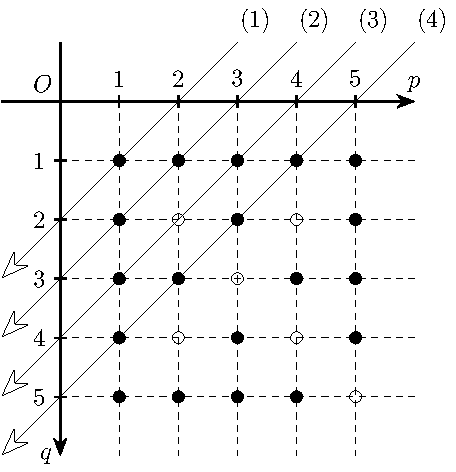
\includegraphics[width=0.5\linewidth]{rational_countable.pdf}
    \caption{
        正の有理数に番号をつける方法.
        まず図のように格子をかき,正の有理数$p/q$に対応する点を黒く塗る.
        次に(1)のように線を引くと,有理数$1/1 = 1$があるので,これを1番目の有理数とする.
        続けて(2)の線を引くと,有理数$2$と$1/2$があるので,それぞれ順に2番目と3番目の有理数とする.
        これを(3),(4)と繰り返すと,正の有理数すべてに番号がつけられる.
    }
    \label{fig:positive-rational-count}
\end{figure}


\begin{proof}
    まず,正の自然数に\cref{fig:positive-rational-count}の方法で番号をつけると,
    \[  1, \ 
        2, \ \frac{1}{2}, \ 
        3, \ \frac{1}{3}, \ 
        4, \ \frac{2}{3}, \ \frac{3}{2}, \ \frac{1}{4}, \ 
        \dotsc  \]
    となる.これを正負交互に並べる.すると
    \[  \overset{1}{0}, \ 
        \overset{2}{1}, \ \overset{3}{-1}, \ 
        \overset{4}{2}, \ \overset{5}{-2}, \ \overset{6}{\frac{1}{2}}, \ \overset{7}{-\frac{1}{2}}, \ 
        \overset{8}{3}, \ \overset{9}{-3}, \ \dotsc  \]
    となる.このようにして有理数と番号(自然数)が1対1に結び付く.
\end{proof}



\begin{theorem}
    実数全体の集合$ℝ$は非可算無限集合である\cite[\S 7]{uchida-set-2020}.
\end{theorem}

\begin{proof}
    $(0, 1] \subset ℝ$が非可算であることを示せば十分である.
    まず$(0, 1]$は明らかに有限集合ではない.
    そこで,$(0, 1]$が\refdfn-[可算無限集合]{dfn:countably-infinite}であると仮定する.
    $(0, 1]$の元(つまり$0$より大きく$1$以下の実数)が自然数で$x_1, x_2, \dotsc$とラベル付けされるので,
    それぞれ小数展開して
    \begin{align*}
        x_1 &= 0.c_{11}c_{12}c_{13}c_{14}c_{15}\dotso \\
        x_2 &= 0.c_{21}c_{22}c_{23}c_{24}c_{25}\dotso \\
        x_3 &= 0.c_{31}c_{32}c_{33}c_{34}c_{35}\dotso \\
        &\vdots 
    \end{align*}
    のように並べる\footnote{
        このとき,有限小数$0.2$は$0.19999\dotso$のように無限小数になるように表記する.
        こうすることで,小数展開が一意になる\cite[\S 7]{uchida-set-2020}.
    }.
    ここで
    \begin{equation*}
        y \coloneq 0. a_1 a_2 a_3 a_4 a_5 \dotso;
            \quad a_i \coloneq
            \begin{cases}
                1  &  \text{if } c_{ii}   =  0  \\
                0  &  \text{if } c_{ii} \neq 0
            \end{cases}
    \end{equation*}
    は明らかに$(0, 1]$の元であるが,
    どの$x_i$とも(小数点以下$i$桁目が)一致しない.
    したがって$(0, 1]$が可算であるという仮定が誤りである\cite[\S 7]{uchida-set-2020}.
\end{proof}



\begin{proposition}
    \label{thm:countable-subset}
    任意の無限集合は,\refdfn-[可算無限]{dfn:countably-infinite}である部分集合を持つ.
\end{proposition}

\begin{proof}
    無限集合$X$からある元$x_1$をとる.
    次に,$X \setminus \{ x_1 \}$から元$x_2$を適当に選んでとる.
    さらに,$X \setminus \{ x_1, x_2 \}$から元$x_3$をとる.
    $X$は無限集合ゆえ,この操作を無限回繰り返すことができる%
    \footnote{
        ここで,無限集合から元をえらぶという操作を無限回行っている.
        この操作が可能であることは,実は選択公理によって保障される.
        選択公理は基底の存在定理の証明でも用いられる,
        数学で最も基本的な(そして最も議論をよんだ)公理のひとつである.
    }.
    このように構成された集合$\{ x_1, x_2, x_3, \dotsc \}$は可算無限集合である.
\end{proof}


\begin{corollary}
    可算無限は,無限の中で最も小さい.
\end{corollary}

\begin{proof}
    \cref{thm:countable-subset}より,
    任意の無限集合が可算無限集合を含む,
    すなわち無限の大きさは可算無限以上であることから従う.
\end{proof}



\begin{proposition}
    $\symbb{N} \times \symbb{N}$は可算無限である.
    より一般に,$\underbrace{\symbb{N} \times \dots \times \symbb{N}}_{\text{有限個}}$
    は可算集合である.
\end{proposition}

\begin{proof}
    $\symbb{N} \times \symbb{N}$が可算であることは,
    \cref{fig:positive-rational-count}とまったく同じ手順で示される.
\end{proof}


この節で最も重要なのは,
無限の中にもレベルがあるということである.
すなわち,
\begin{enumerate}
    \item 有限個
    \item 可算無限個(たとえば$\symbb{N}$,$\symbb{Q}$,$\symbb{N} \times \symbb{N}$)
    \item 非可算無限個(たとえば$ℝ$)
\end{enumerate}
可算であるか非可算であるかの区別は重要である.




\subsection{同値類}

有理数$1/3$と$2/6$は,見た目こそ違うが同じ数である.
このようなものを「同じ」として扱う方法が\ruby{同値類}{どう|ち|るい}である.

まず同値関係について見る.

\begin{definition}[二項関係]
    \label{dfn:binary-relation}
    $X$を集合とする.
    規則$\mathbin{\rho}$が$X$上の\word{二項関係}(binary relation)であるとは,
    任意の$x, y \in X$に対し,$x \mathbin{\rho} y$が満たされるか満たされないかを判別できるときをいう.
\end{definition}

\begin{example}
    不等号$<$は$ℝ$上の二項関係である.
    実際,任意の$a, b \in ℝ$に対し,$a<b$が真であるか偽であるかを判別できる.
\end{example}


\begin{definition}[同値関係]
    \label{dfn:equivalence-relation}
    $X$を集合とする.
    $X$上の二項関係$\sim$が\word{同値関係}(equivalence relation)であるとは,以下をすべて満たすことをいう.
    \begin{enumerate}
        \item (\word{反射律}(reflexivity))任意の$x, y \in X$に対し,$x \sim x$である.
        \item (\word{対称律}(symmetry))任意の$x, y \in X$に対し,$x \sim y$ならば$y \sim x$である.
        \item (\word{推移律}(transitivity))任意の$x, y, z \in X$に対し,$x \sim y$かつ$y \sim z$ならば$x \sim z$である.
    \end{enumerate}
\end{definition}

\begin{example}
    任意の集合$X$に対して,$=$は$X$上の自明な同値関係である.
\end{example}

\begin{example}
    $ℂ$上の二項関係$\sim$を
    \begin{equation*}
        x \sim y  \iff  \abs{x} = \abs{y}
    \end{equation*}
    で定めると,$\sim$は同値関係である.
\end{example}


この同値関係を使って,同値類というものを定義できる.

\begin{definition}[同値類]
    \label{dfn:equivalence-class}
    $X$を集合,$\sim$を$X$上の同値関係とする.
    $x \in X$に対し,
    \begin{equation}
        \eqclass{x}  \coloneq  \Set{ y \in X  \given  x \sim y } \subset X
    \end{equation}
    を元$x$の\word{同値類}[どう|ち|るい](equivalence class)という.
    また,$x$のことを同値類$\eqclass{x}$の\word{代表元}[だい|ひょう|げん](representative)という.
\end{definition}

\begin{definition}[商集合]
    \label{dfn:quotient-set}
    $X$を集合,$\sim$を$X$上の同値関係とする.
    同値類全体の集合
    \begin{equation}
        X/{\sim} \coloneq \Set{ \eqclass{x} \subset X  \given  x \in X }
    \end{equation}
    を\word{商集合}[しょう|しゅう|ごう](quotient set)という,
\end{definition}


\begin{example}
    $\symbb{Z}$に対し,同値関係$\sim$を
    \begin{equation*}
        x \sim y  \iff  \text{$x-y$が$3$で割りきれる}
    \end{equation*}
    で定める.
    つまり,$x$を3で割ったときの余りと$y$を5で割ったときの余りが同じであるとき,$x \sim y$とする.
    たとえば,$0 \sim 3 \sim 6 \sim \dotsb$であり,$-1 \sim 2 \sim 5 \sim \dotsb$である.
    したがって同値類は,
    \begin{align*}
           \eqclass{0} &= \{ \dotsc, -3, 0, 3, 6, 9, \dotsc \}
        &  \eqclass{1} &= \{ \dotsc, -2, 1, 4, 7, 10, \dotsc \}
        \\ \eqclass{2} &= \{ \dotsc, -1, 2, 5, 8, 11, \dotsc \}
    \end{align*}
    であり,商集合$\symbb{Z}/{\sim} = \{ \eqclass{0}, \eqclass{1}, \eqclass{2} \}$である
    \footnote{この場合の商集合を特に$\symbb{Z}/3$とかくこともある}.
    
    また,$\eqclass{0} = \eqclass{3} = \eqclass{6} = \dotsb$.
    このことからわかるように,1つの同値類に対する\emph{代表元の取り方は一般に一意ではない}.

    明らかに$\symbb{Z} = \eqclass{0} \sqcup \eqclass{1} \sqcup \eqclass{2}$であり,同値類が互いに交わらずに$\symbb{Z}$を分割している.
\end{example}


例で見た「同値類が互いに交わらずに集合を分割する」ことは,一般の集合においても成り立つ.
\begin{theorem}
    同値関係$\sim$が定義された集合$X$は,同値類によって互いに交わらない部分集合に分割される.
    すなわち適当な$x_1, x_2, \dotsc \in X$を用いて
    \begin{equation*}
        X = \bigsqcup_{\lambda \in \Lambda} \eqclass{x_\lambda}
            \quad \text{(\refdfn[非交和]{dfn:disjoint-union})}
    \end{equation*}
\end{theorem}

\begin{proof}
    $X = \bigcup_{\lambda \in \Lambda} \eqclass{x_\lambda}$は明らかなので,非交和であることを示す.
    $\eqclass{x} \cap \eqclass{y} \neq \emptyset$なら$\eqclass{x} = \eqclass{y}$を示せばよい.

    そこで$z \in \eqclass{x} \cap \eqclass{y}$とする.
    $z \in \eqclass{x}$より$x \sim z$であり,
    $z \in \eqclass{y}$なので$y \sim z$である.
    $\sim$の対称律と推移律を用いると,$x \sim y$がいえる.
    したがって$\eqclass{x} = \eqclass{y}$である.
\end{proof}


\subsection{便利な記号}

この節では,数式を扱ううえで便利な記号を導入する.

\begin{definition}[クロネッカーのデルタ]
    \label{dfn:Kronecker-delta}
    次で定義される$\delta_{i, j}$を\word{クロネッカーのデルタ}という:
    \begin{equation}
        \delta_{i, j} = 
            \begin{cases}
                1  &  \text{if } i  =   j ,  \\
                0  &  \text{if } i \neq j .
            \end{cases}
    \end{equation}
\end{definition}



\end{document}

